\chapter{The ASK corpus}

In this chapter we will describe the data set used throughout the thesis. The
process used to select the split between training, testing and validation
data is also described.


\section{Data set}

% cspell:disable
The ASK corpus (\emph{andrespråkskorpus}) was presented in 2006
\autocite{tenfjord06}. The corpus contains Norwegian learner essays from two
different language tests: \emph{Språkprøven i norsk for voksne innvandrere}
and \emph{Test i norsk – høyere nivå}. The two test levels are not offically
tied to the CEFR framework, but \textcite{carlsen2012proficiency} estimated
them to measure proficiency at approximately B1 and B2/C1 level,
respectively. Following the naming in \textcite{carlsen2012proficiency}, we
will refer to these tests as the \emph{IL test} (Intermediate Level,
``Språkprøven'') and the \emph{AL test} (Advanced Level, ``Høyere nivå'').
% cspell:enable

\begin{table}
  \centering
  \begin{tabular}{lrrr}
    \toprule
    First language             & IL test & AL test & Total \\
    \midrule
    English                    &     100 &     100 &   200 \\
    Polish                     &     100 &     100 &   200 \\
    Russian                    &     100 &     100 &   200 \\
    Somali                     &     100 &       7 &   107 \\
    Spanish                    &     100 &     100 &   200 \\
    German                     &     100 &     100 &   200 \\
    Vietnamese                 &     100 &       5 &   105 \\
    \midrule
    Subtotal (included languages) &  700 &     512 &  1212 \\ \addlinespace
    \midrule
    (Albanian)                 &     100 &      24 &   124 \\
    (Bosnian-Croatian-Serbian) &     100 &     100 &   200 \\
    (Dutch)                    &     100 &     100 &   200 \\
    (Norwegian nynorsk)        &      11 &      21 &    32 \\
    (Norwegian bokmål)         &      89 &      79 &   168 \\
    \midrule
    Subtotal (excluded languages) &  400 &     324 &   724 \\ \addlinespace
    \midrule
    Total (all languages)      &    1100 &     836 &  1936 \\
    \bottomrule
  \end{tabular}
  \caption[Distributions of first languages for each test level in ASK]{
    Texts in each test level for all \acp{L1}. Languages which are
    left out of our AES dataset are listed in round brackets.
  }
  \label{tab:l1-and-testlevel}
\end{table}

The corpus contains 1736 texts\footnote{In
\textcite{carlsen2012proficiency,malmasi15,malmasi17}, it's reported that it
contains 1700 texts.}. Each document includes metadata such as the writer's
L1: one of German, Dutch, English, Spanish, Russian, Polish,
Bosnian-Croatian-Serbian, Albanian, Vietnamese and Somali. All texts from
seven of these language backgrounds, 1212\footnote{Reported to be 1222 in
\textcite{carlsen2012proficiency}.} in total, have been assigned a \ac{CEFR}
score, and these texts comprise the subcorpus we will be working with. In
particular, all texts except those written by people with Dutch,
Bosnian-Croatian-Serbian or Albanian as L1 have a CEFR score. The CEFR labels
are available since work by \textcite{carlsen2012proficiency}, and were not
included at the corpus' initial release. Table \ref{tab:l1-and-testlevel}
shows the number of texts in the corpus for each native language and at each
test level.

Among the languages we include, there are five languages from the
Indo-European language family. Breaking them further down into branches,
there are two Germanic (English and German), two Slavic (Polish and Russian),
and one Italic language, Spanish. Finally, there is one Afro-Asiatic
language, Somali, and one Austroasiatic, Vietnamese.

The corpus also includes 200 texts written by native Norwegian speakers as a
control corpus, bringing the total number of documents up to 1936. The total
number of word and punctuation tokens in the full corpus, including the
control corpus, is approximately 770,000. Restricting the corpus to the 1212
documents with \ac{CEFR} score, the number of tokens is approximately 487,000
in total. Other metadata, apart from L1 and CEFR score, includes, but are not
limited to: the test level the essay was written for, what topic the essay
is about, and the learner's country of origin, age, and gender.

The CEFR scores in the ASK corpus range between A2 and C1, and also includes
intermediate labels between the canonical proficiency scores, such as A2/B1
and B1/B2. Thus, the total number of distinct CEFR scores is seven, which is
more fine-grained than the TOEFL11 corpus \autocite{blanchard13}, which uses
three distinct proficiency categories, not necessarily corresponding to CEFR
scores. The corpus used in \textcite{vajjala18universalCEFR}, the MERLIN
corpus, has CEFR scores ranging between A1 and C1, but does not use any
intermediate levels.

As mentioned, the two test levels making up the ASK corpus are estimated to
measure proficiency at the B1 and B2/C1 levels in the CEFR framework.
However, many essays are rated with CEFR scores both above and below the
estimated level of their associated test. Essays scoring higher are easily
accounted for, considering that a learner at a high level is expected to pass
a test at a lower level. The essays scoring below the test level can also be
accounted for, even though we know that all the documents in ASK are taken
from learners who passed their test. First, while ASK only contains essays,
the original test consisted of multiple parts, and a low score on the essay
part could be outweighed by good performance by the learner on other parts of
the test. Second, the CEFR labels in ASK were assigned after the test, by
different raters, who cannot be expected to be in complete agreement with the
raters who originally passed the tests.

The fine-grained labels makes it challenging to train and evaluate models,
and also to compare the results against work on other corpora, because the
gravity of a misclassification may not the same on the more fine-grained
labels.


\subsection{Examples}

As an example of texts in the ASK corpus, we give an excerpt from a text from
the corpus. This is a paragraph from a text written by a native English
speaker from Australia. The author was taking the IL test, and was given the
prompt ``Skriv en tekst om nyheter'' (\emph{Write a text about the news''}).
The text was assessed to be on level `B2/C1' in the CEFR framework.

\begin{displayquote}  % ASK: s0354
  % cSpell: disable
  Når jeg tenker på ordet ``nyheter'' så tenker jeg automatisk på (de)
  massemediene og hvordan vi alminnelige mennesker få vite (om) de store
  hendelsene i verden vår. Jeg pleier å se nyheter på TV og å lese aviser, og
  jeg synes at nyheter kan gjøre et veldig sterkt inntrykk på oss. Et
  eksempel på dette er de forstillingsbildene av andre land og kulturer som
  nyheter i mediene påvirker oss til å skape.
  % cSpell: enable
\end{displayquote}


\subsection{Features of learner language}

The ASK corpus has been used in several studies on features Norwegian learner
language and transfer effects from different \acp{L1}.

\textcite{pepper2012} uses predictive analysis to find lexical features that
are indicative of different \acp{L1}. The study was designed to closely
replicate \textcite{jarvis}, which influenced many of the methodological
design decisions. In the study, experiments were limited to different subsets
of five languages. All features were based on word counts. The predictive
model used was \acp{LDA}.

Concrete findings from the \citeauthor{pepper2012} study include that
learners with a Slavic language background (Russian and Polish) used
indefinite articles (`en', `et' and `ei' in Norwegian bokmål) less
frequently. This was interpreted as cross-linguistic transfer, since the
relevant \acp{L1} lack indefinite articles. The study found multiple
distinguishing patterns in the use of prepositions, but providing possible
explanations for the differences was out of its scope. These two patterns
serve here as indicative of the results of the study regarding transfer
effects, but they are far from an exhaustive account of the findings.

In \textcite{golden2016ask}, the author examines the different uses of a
specific verb in the ASK corpus. Specifically, the verb `gjøre', which
corresponds to the English `do' or `make'. The study uses a subset of the
corpus, only looking at texts from learners with English, German, Polish or
Spanish as their \ac{L1}. The occurrences of the verb are categorized into
different cases based on the different semantic functions of the verb.

A finding from the study is that the overall relative frequency of the verb
differs between the different language groups. There were also patterns at
the level of each semantic function of the verb.

Another study \autocite{vigrestad2016} which also is based on the ASK corpus
looks at orthographical mistakes in Norwegian learner language. The author
considered two language groups from the ASK corpus: learners with
Bosnian-Serbian-Croatian or Vietnamese as \ac{L1}. Several different
categories of mistakes were considered in the study, including the general
prevalence of mistakes per word of running text, groups of consonant
graphemes and mistakes involving single and double consonants.

Several of the differences discovered in the study were statistically
significant. The author also interpreted the differences in terms of transfer
effect from \ac{L1} on \ac{L2}. For instance, mistakes in substituting the
vowel graphemes `i' and `y' can often be seen in texts where the author's L1
has no phonological distinction between the vowel sounds [i] and [y], as is
the case in, for instance, Bosnian-Serbian-Croatian.


\subsection{Analyzing non-linguistic variables}

\begin{figure}
  \centering
  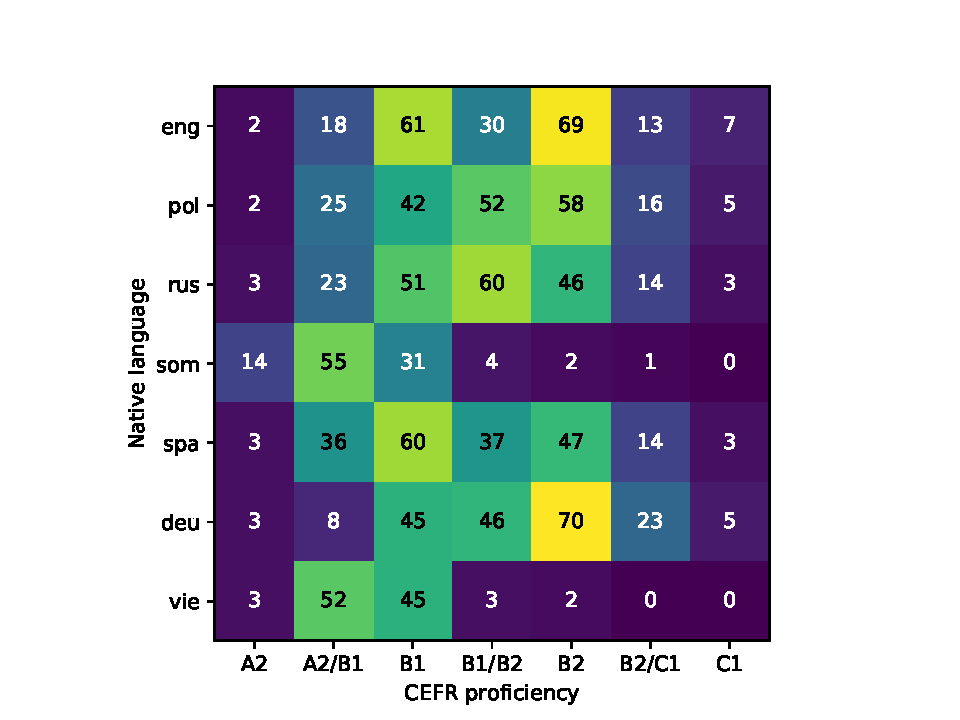
\includegraphics{lang_vs_cefr}
  \caption{The distribution of proficiency scores for each L1}
  \label{fig:lang-vs-cefr}
\end{figure}
 
\begin{figure}
  \centering
  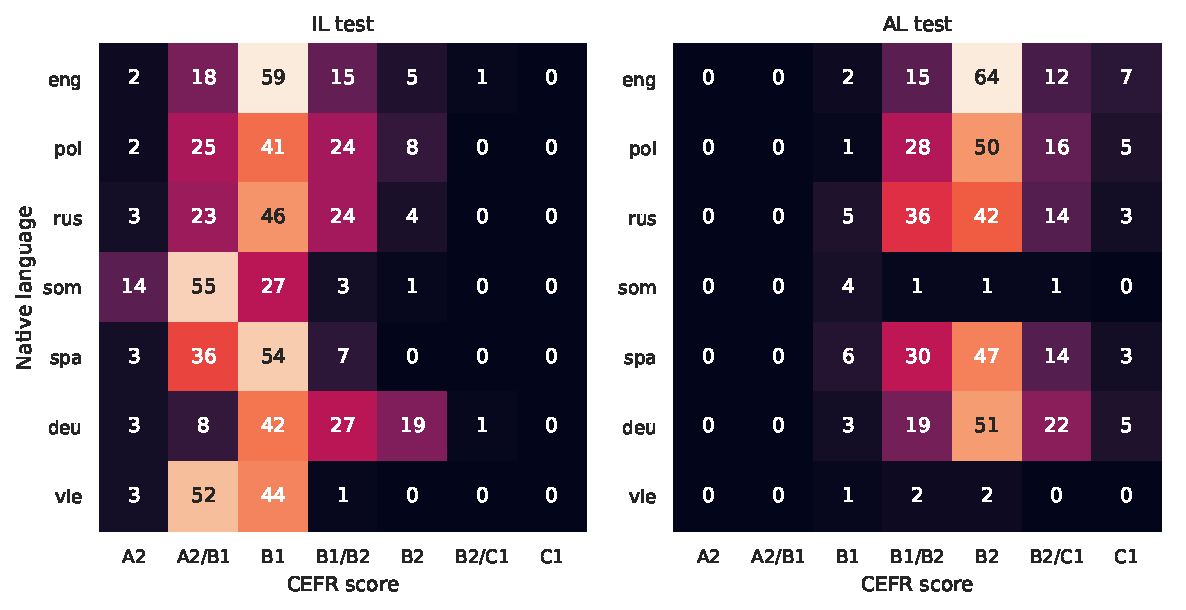
\includegraphics{testlevel_lang_vs_cefr}
  \caption{L1 versus CEFR score for each test level}
  \label{fig:testlevel-lang-vs-cefr}
\end{figure}

We analyze the data set in order to find correlations between different
metadata. Knowing that the documents stem from two different language tests
that measure different levels of proficiency, the data set was split in two
using the \emph{Test level} label, and then broken down by language and
proficiency again. Figure \ref{fig:testlevel-lang-vs-cefr} shows that the
test levels have different distributions of proficiency. Note also that two
language groups are underrepresented at the B2 test level (\emph{AL test}),
namely Somali and Vietnamese, which have seven and five essays in the B2 test
level, respectively. All other combinations of L1 and test level contain
exactly 100 essays. This partly explains the low average proficiency of
Somali and Vietnamese speakers apparent in figure \ref{fig:lang-vs-cefr}. The
difference compared to the other language groups is less salient when looking
only at the B1 test level (\emph{IL test}) data (figure
\ref{fig:testlevel-lang-vs-cefr}, left).

In fact, the distribution of CEFR scores corresponds to the similarity of the
various \acp{L1} to Norwegian. The Germanic languages, German and English,
have the fewest number of essays below B1 level in the IL test. The
non-Indo-European languages, Vietnamese and Somali, rarely score above B1
level in the IL test, and their mode is A2/B1 compared to B1 for all the
Indo-European languages.

\begin{table}
  \centering
  \begin{tabular}{lrrr}
    \toprule
    Topic                    & IL test & AL test & Total \\
    \midrule
    % cspell:disable
    telefon                  &      64 &      37 &   101 \\
    bolig                    &      83 &       0 &    83 \\
    familie helse vekt       &       0 &      59 &    59 \\
    tid                      &      51 &       2 &    53 \\
    natur norge              &      48 &       0 &    48 \\
    folk relasjoner vennskap &      45 &       0 &    45 \\
    tradisjoner flytting     &      38 &       0 &    38 \\
    barn                     &      32 &       3 &    35 \\
    kultur norge             &      34 &       0 &    34 \\
    media                    &      31 &       0 &    31 \\
    % cspell:enable
    \bottomrule
  \end{tabular}
  \caption[Most common topics in ASK texts]{
    The number of texts in each test level for the top 10 topics
    across test level.
  }
  \label{tab:texts-per-topic}
\end{table}

Another interesting variable is the essay topic. When we refer to the topic,
we refer to the `tema' (theme, topic) variable in the documents' metadata
section, as opposed to the essay title, for instance. The various prompts do
not correspond strictly to topic.

We can generally expect a high correlation between topic and vocabulary, and
not accounting for this may lead to a model picking up the wrong signal.
Since the data is collected from two different language tests, we might
expect the distribution of topics to differ between the test levels, and this
is indeed the case. Looking at the ten most common topics in the data (table
\ref{tab:texts-per-topic}), several are only present on one test level.

There is also a difference in granularity. There are 52 different topics in
the AL test, and only 38 topics in IL test, even though there are more
documents in the latter test level (512 vs. 700). This also means that the
topics within each test level have different support. The median number of
documents for a topic in AL test is 5 (mean $9.8$), while it is 11 in IL test
(mean $18.4$). This also explains the overrepresentation of the IL test in
the table of top ten topics. The individual topics in the AL test have fewer
occurrences, and thus are less likely to appear on the top ten list when we
combine the test levels.

% cspell:disable
It has been observed that some topics in the diagram consist of several
sub-topics (for instance, ``natur norge'' consists of ``natur'' and
``norge''). However, the number of individual sub-topics is 62, still quite
large. However, they seem to be more evenly distributed across essays. The
median number of documents for a sub-topic, for both test levels, is 25 (mean
$34.8$). 13 sub-topics are only represented in 5 or fewer documents.
% cspell:enable

\begin{figure}
  \centering
  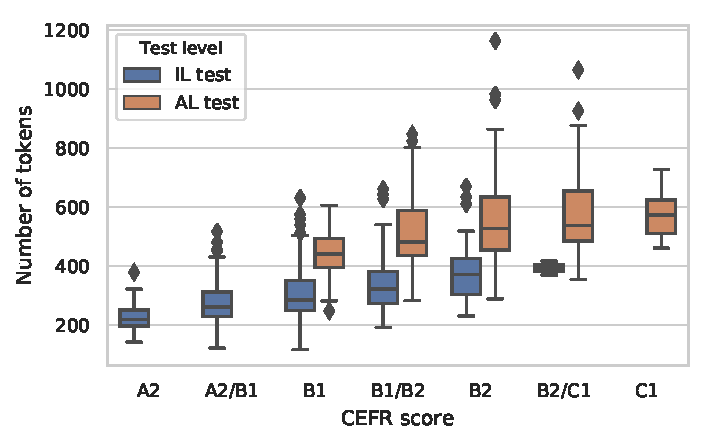
\includegraphics{testlevel_lengths_per_cefr}
  \caption[Document lengths on each CEFR level]{
    Distributions of essay lengths for CEFR scores on each test level.
  }
  \label{fig:testlevel-lengths-per-cefr}
\end{figure}

Document lengths have been seen to correlate with essay score in other
studies such as \textcite{vajjala17}. To see the relationship between these
variables in ASK, we again break down the data into the two test levels. One
group, \emph{B2/C1} CEFR score within \emph{IL test}, was excluded due to
having fewer than ten documents. Looking at figure
\ref{fig:testlevel-lengths-per-cefr}, two relations are apparent. Essays in
the \emph{AL test} test level are generally longer than in \emph{IL test},
and within each test level the higher scoring essays are generally longer.
Also, outliers are generally on the long side.

Note that even for the same CEFR score, the essays from the higher test level
are considerably longer. As an example, consider the \emph{B1/B2} score,
which is the most evenly distributed between the two test levels (101 essays
in \emph{IL test}, 131 in \emph{AL test}). More than 75\% of these texts on
the lower test level have fewer than 400 tokens, and more than 75\% on the
higher level are longer than 400 tokens. In fact, for all four CEFR scores
that are present on both test levels, there is no overlap of the
interquartile ranges\footnote{The range of values when the top 25\% and
bottom 25\% are excluded} between IL and AL test level.


\section{Data split}

At the start of the project, the dataset was split into a training,
development and test set in a 8:1:1 proportion. Ideally, the train and test
sets would have the same distribution of classes, but the limited amount of
data made this more difficult. As can be seen from figure
\ref{fig:lang-vs-cefr}, 15 of the combinations language vs. proficiency label
consist of only three or fewer documents.

Moreover, we wanted each split to consist of text topics not present in the
other splits. The reason for this to prevent a model from learning a bias for
topic. Finding a split that satisfies our constraints is an optimization
problem for which it can be intractable to find an optimal solution. We
therefore turned to heuristics, hoping that it would help us find a good
local optimum.
 
The split was chosen in order to have the right proportion of documents in
each part of the split, and so the distribution of proficiency and native
language is as similar as possible across the separate parts of the data
split. Specifically, the split was found by running an evolutionary algorithm
with a fitness function favouring splits that were as close as possible to
8:1:1 in proportion, while ensuring that each split contained a disjoint set
of topics.

We designed a fitness function incurred several penalties. A candidate split
was given a size penalty proportional to the absolute difference between the
sizes of test and dev splits and the wanted size, namely 10\% of the corpus.
Further, we added a label distribution penalty by calculating the
Kullback-Leibler divergences between the distributions of CEFR and L1 labels
in the candidate splits and the distribution in the entire corpus.
Kullback-Leibler divergence was computed using the SciPy \autocite{scipy}
library. The divergence values were squared and added to the penalty.

\begin{table}
  \centering
  \begin{tabular}{ll}
    \toprule
    Topics in development set &       Topics in test set \\
    \midrule
    % cspell:disable
         idrett/sport kultur &       geografi norge folk \\
                organisasjon &               innvandring \\
                  opplevelse & innvandring politikk valg \\
                     økonomi &              idrett/sport \\
                    holdning &            bolig geografi \\
           barn idrett/sport &               arbeid yrke \\
            familie flytting &          økonomi holdning \\
               eldre familie &              humor kultur \\
               helse røyking &   politikk norge holdning \\
       litteratur dikt språk &            litteratur bok \\
    helse arbeid innvandring &  familie befolkning norge \\
                barn familie &    litteratur dikt idrett \\
                       helse &           folk utdannelse \\
            utdannelse språk &         politikk holdning \\
          arbeid innvandring &                  media tv \\
      litteratur dikt venner &                  religion \\
                             &               helse organ \\
                             &             folk følelser \\
    % cspell:enable
    \bottomrule
  \end{tabular}
  \caption[Essay topics in development and test sets]{
    The topics chosen to be in each of the development and test sets.
  }
  \label{tab:topics-in-split}
\end{table}

% cspell:disable
The split in terms of the topics can be seen in table
\ref{tab:topics-in-split} \footnote{In the XML files, the topic values
contain a trailing space character, not visible in print.}. The dev and test
sets contain 123 texts each, close to the ideal 10\% of the corpus, which is
121. The topic variable has values which are sets of keywords, and therefore
there is still topical overlap between splits. For example, `økonomi'
(economy) and `økonomi holdning' (economy attitude) are considered separate
values and assigned to different splits, even though both topics include the
`economy' keyword.
% cspell:enable

\begin{figure}
  \centering
  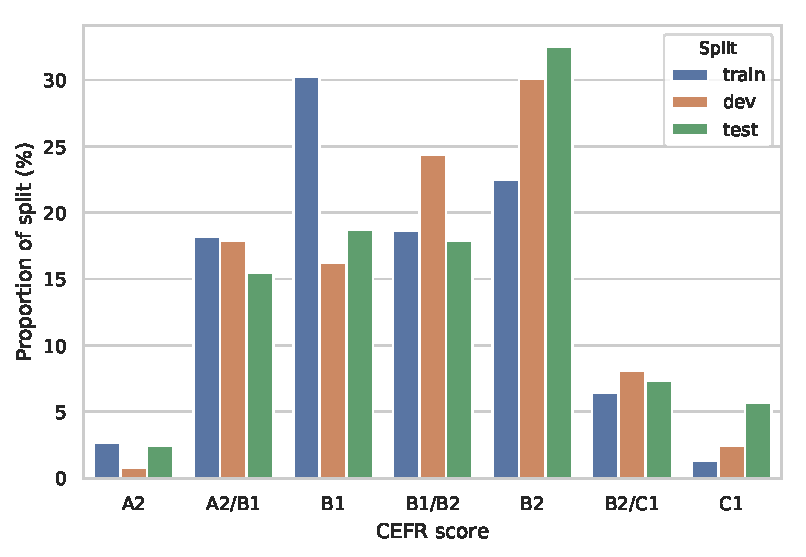
\includegraphics[width=\textwidth]{split-cefr-dist}
  \caption{Proportional distribution of CEFR labels in the three splits.}
  \label{fig:split-cefr-dist}
\end{figure}

\begin{figure}
  \centering
  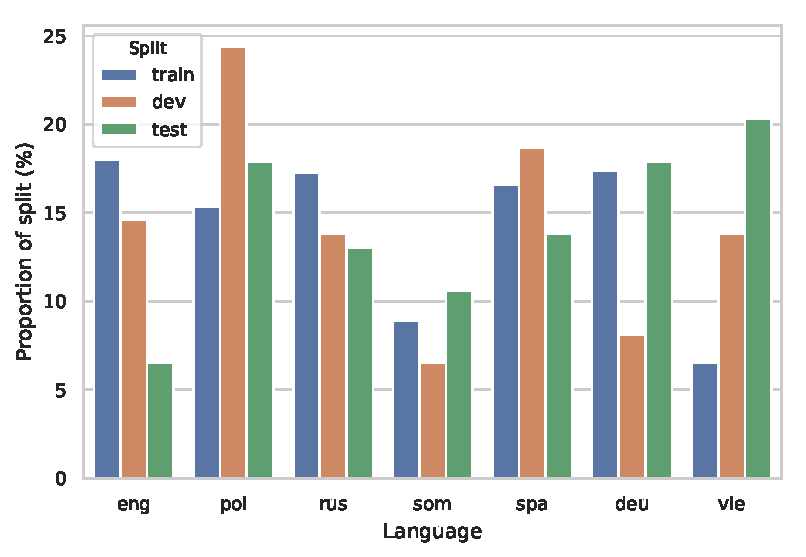
\includegraphics[width=\textwidth]{split-lang-dist}
  \caption{Proportional distribution of language labels in the three splits.}
  \label{fig:split-lang-dist}
\end{figure}

Figure \ref{fig:split-cefr-dist} shows how CEFR labels are distributed in the
resulting training, development and test splits, and figure
\ref{fig:split-lang-dist} shows the same for language labels. It can be seen
that all splits contain texts on all CEFR levels and for all different
\acp{L1}. While there are considerable differences in the distributions, we
decided that the result was reasonable given the constraints and the small
size of the dataset.

Each split does not contain every combination of CEFR score and \ac{L1}. This
follows from the distribution plotted in figure \ref{fig:lang-vs-cefr}, where
we find five combinations of CEFR score and \ac{L1} that occur only once or
twice. Since each document is assigned to exactly one of three different
splits, these combinations must necessarily be absent from one or two of the
splits.
